%
% iteration.tex -- template for standalon tikz images
%
% (c) 2019 Prof Dr Andreas Müller, Hochschule Rapperswil
%
\documentclass[tikz]{standalone}
\usepackage{amsmath}
\usepackage{times}
\usepackage{txfonts}
\usepackage{pgfplots}
\usepackage{csvsimple}
\usetikzlibrary{arrows,intersections,math}
\begin{document}
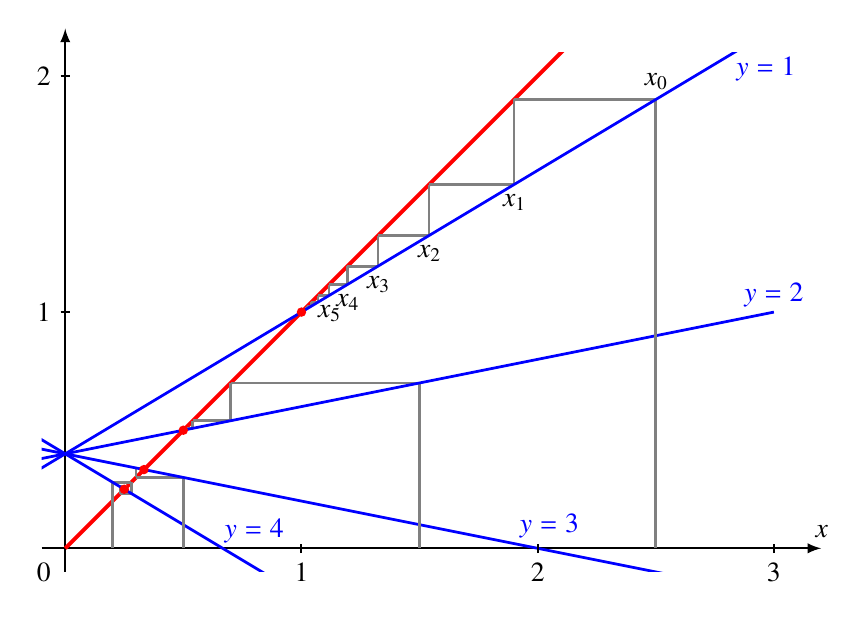
\begin{tikzpicture}[>=latex,scale=3]

\def\maxx{3}
\def\maxy{2}

\draw[->,line width=0.7pt] (-0.1,0)--({\maxx+0.2},0) coordinate[label={$x$}];
\draw[->,line width=0.7pt] (0,-0.1)--(0,{\maxy+0.2});
%coordinate[label={left:$x^{-1}$}];

\begin{scope}
\clip (-0.1,-0.1) rectangle ({\maxx+0.1},{\maxy+0.1});

%\draw[color=black,line width=1pt] plot[domain=0.2:6,samples=100] ({\x},{1/\x});

\draw[line width=1.4pt,color=red] (0,0)--(\maxx,\maxx);

\def\A{5}
\def\B{1}
\pgfmathparse{2/(\A*\B)}
\xdef\c{\pgfmathresult}

\def\gerade#1#2{

	\xdef\xold{#2}
	\xdef\yold{0}

	\foreach \i in {1,...,15}{
		\xdef\x{\xold}
		\pgfmathparse{\x+(\c)*(1-\x*#1)}
		\xdef\y{\pgfmathresult}

		\draw[line width=1pt,color=gray] ({\xold},{\yold})--({\x},{\y});

		\xdef\xold{\x}
		\xdef\yold{\y}
		\xdef\x{\y}

		\draw[line width=1pt,color=gray] ({\xold},{\yold})--({\x},{\y});

		\xdef\xold{\x}
		\xdef\yold{\y}
	}

	\draw[line width=1.0pt,color=blue]
		(-1,{-1+(\c)*(1+#1)})--(\maxx,{\maxx+(\c)*(1-(\maxx*#1))});

}

\gerade{4}{0.2}
\gerade{3}{0.5}
\gerade{2}{1.5}
\gerade{1}{2.5}

\def\punkt#1{
	\fill[color=red] ({#1},{#1}) circle[radius=0.02];
}

\punkt{0.25}
\punkt{0.3333}
\punkt{0.5}
\punkt{1}

\end{scope}

\xdef\xold{2.5}
\xdef\yold{0}

\xdef\x{\xold}
\pgfmathparse{\x+(\c)*(1-\x*1)}
\xdef\y{\pgfmathresult}

\xdef\xold{\x}
\xdef\yold{\y}

\node at ({\xold},{\yold}) [above] {$x_0$};

\xdef\x{\y}

\xdef\xold{\x}
\xdef\yold{\y}

\foreach \i in {1,...,5}{
	\xdef\x{\xold}
	\pgfmathparse{\x+(\c)*(1-\x*1)}
	\xdef\y{\pgfmathresult}

	\xdef\xold{\x}
	\xdef\yold{\y}
	\xdef\x{\y}

	\node at ({\xold},{\yold}) [below] {$x_\i$};

	\xdef\xold{\x}
	\xdef\yold{\y}
}

\foreach \x in {1,...,\maxx}{
	\draw[line width=0.7pt] ({\x},{-0.02})--({\x},{0.02});
	\node at ({\x},{-0.02}) [below] {$\x$};
}

\foreach \x in {1,...,\maxy}{
	\draw[line width=0.7pt] ({-0.02},{\x})--({0.02},{\x});
	\node at ({-0.02},{\x}) [left] {$\x$};
}

\node at (-0.02,-0.02) [below left] {$0$};

\node[color=blue] at (0.8,-0.02) [above] {$y=4$};
\node[color=blue] at (2.05,0) [above] {$y=3$};
\node[color=blue] at (3,0.98) [above] {$y=2$};
\node[color=blue] at (2.8,2.03) [right] {$y=1$};

\end{tikzpicture}
\end{document}

